\pagestyle{fancy}
\setlength{\headheight}{16pt}
\fancyhead{} % clear all header fields
\fancyhead[L]{\textbf{TAM 514 Homework 2}}
\fancyhead[C]{Songyuan Cui}
\fancyhead[R]{\textbf{Spring 2025}}
\fancyfoot{} % clear all footer fields
\fancyfoot[C]{\thepage}

\begin{problem}
\textbf{1 (150 pts).} (After an idea of Richard Weaver) Consider the following suspended uniform string hanging under its own weight. 
Gravity produces the spatially varying tension $T(x) = \rho g x$, where $x$ is measured from the bottom of the string. 
Ignore other gravitational effects. 
We want to study the oscillations of this string.
\begin{enumerate}[(i)]
    \item {
        Derive the equation of motion using an infinitesimal solid mechanics approach (as shown in class) and formulate carefully the boundary conditions.
    }
    \item {
        Compute the eigenmodes through the following steps:
        \begin{enumerate}[(1)]
            \item {
                Introduce the new independent variable $\xi = kx^n$ (determine $n$) and express the ordinary
                differential equation governing the eigenfunctions as 
                \begin{equation}
                    \xi \frac{d^2 Q }{d\xi^2} + \frac{dQ}{d\xi} + \xi Q = 0
                \end{equation}
            }
            \item {
                Express the general solution of this equation as
                \begin{equation}
                    Q(\xi) = A J_0(\xi) + B Y_0(\xi)
                \end{equation}
                where $J_0(\xi)$ and $Y_0(\xi)$ are Bessel functions of the first and second kind, respectively.
                Now impose the boundary conditions and obtain the equation for the eigenvalues (natural frequencies) and the eigenfunctions of the system. 
                Compute the three leading natural frequencies and corresponding eigenfunctions.
            }
        \end{enumerate}
    }
\end{enumerate}
\end{problem}
\begin{figure}[!ht]
    \centering
    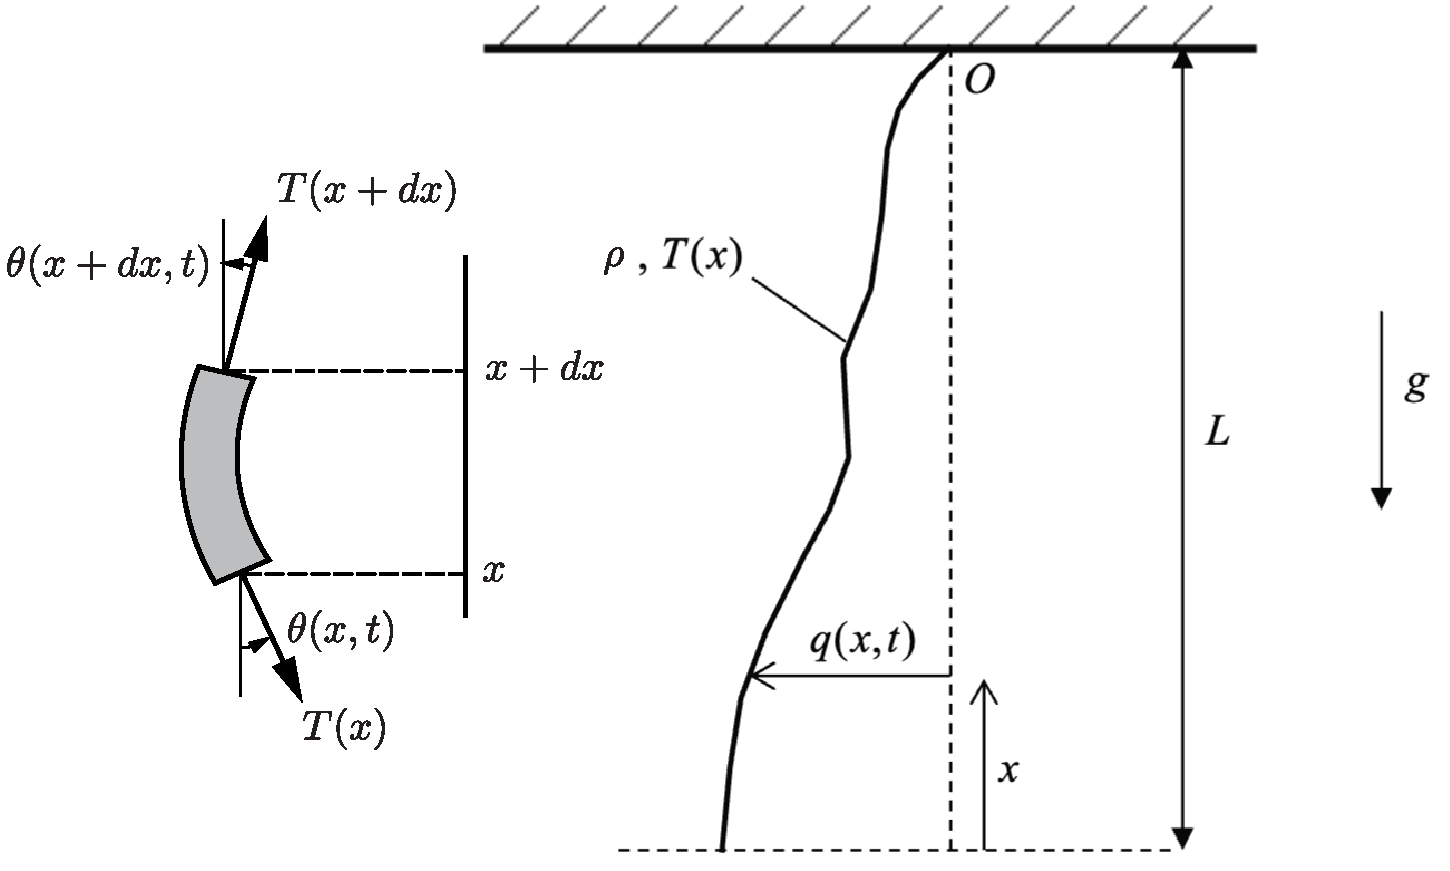
\includegraphics[width=0.6\textwidth]{homework/hw2/assets/hw2_p1.pdf}
    \label{fig:hw2_p1}
\end{figure}
\begin{enumerate}[(i)]
\item { % 1(i)
Consider an infinitesimal element of the string spanning from coordinate $x$ to $x + dx$. 
The the string's rotation from the $x$-direction (vertical) is denoted $\theta(x)$, with a \emph{counter-clockwise rotation being positive}. 
Since we are only considered with the horizontal displacement $q(x,t)$, only the sine-component of the rotation is relevant which, under the assumption of small rotation, is approximated as $\sin(\theta) \approx \tan\theta = \partial q / \partial x$.
Hence, leveraging Newton's laws, 
\begin{equation}
\begin{aligned}
    \rho \frac{\partial^2 q}{\partial t^2}(x, t) dx &= T(x + dx) \sin \left[ \theta(x + dx, t) \right] - T(x) \sin \left[\theta(x, t) \right] \\
    &\approx T(x + dx) \frac{\partial q}{\partial x} \Big|_{x+dx} - T(x) \frac{\partial q}{\partial x} \Big|_{x}
\end{aligned}
\end{equation}
where $\rho$ is the mass of the string per unit length, same as the one used in the tension expression $T(x) = \rho g x$.
Dividing both sides by $dx$ and taking the infinitesimal limit leads to 
\begin{equation}
    \rho \frac{\partial^2 q}{\partial t^2}(x, t) = \lim_{dx \rightarrow 0} \frac{T(x + dx) \frac{\partial q}{\partial x} \Big|_{x+dx} - T(x) \frac{\partial q}{\partial x} \Big|_{x}}{dx} = \rho g \frac{\partial}{\partial x} \left[ x \frac{\partial q}{\partial x} \right]
\end{equation}
wherein we have utilized the definition of derivatives. 
Cancelling $\rho$ on both sides yields the equation of motion 
\begin{equation}\label{eqn:hw2_p1_eom}
    \boxed{\frac{\partial^2 q}{\partial t^2}(x, t) = g \left[ x \frac{\partial^2 q}{\partial x^2} + \frac{\partial q}{\partial x} \right]}
\end{equation}
Assuming $x = 0$ at the bottom of the string, the boundary conditions are 
\begin{equation}
    \boxed{\lim_{x \rightarrow 0} \left[\rho g x \frac{\partial q}{\partial x}(x, t)\right] = 0, ~~~~ q(L, t) = 0}
\end{equation}
where the first condition represents a free boundary condition at the bottom of the string. 
The limit is necessary as the tension $T(x) = \rho g x$ vanishes at $x = 0$, rendering the a non-limit expression trivial. 
The constants $\rho g$ is typically positive and can be cancelled. 
}
\item { % 1(ii)
\begin{enumerate}[(1)]
\item { % 1(ii)(1)
    Define the separable ansatz as 
    \begin{equation}
        q(x, t) = M(x) N(t)
    \end{equation}
    which is substituted into the equation of motion \cref{eqn:hw2_p1_eom} to yield
    \begin{equation}
        M(x) \ddot{N}(t) = g \left[ x M''(x) + M'(x) \right] N(t) ~~~~ \Leftrightarrow ~~~~ \frac{\ddot{N}}{N} = g \frac{x M'' + M'}{M} = -\omega^2
    \end{equation}
    where $\omega$ is the natural frequency, and the negative sign is introduced to ensure an temporally oscillatory solution. 
    This is further separated into a system of two independent ODEs:
    \begin{subequations}
    \begin{align}
        x M'' + M' + \frac{\omega^2}{g} M &= 0 \label{eqn:hw2_p1_M_ode} \\
        \ddot{N} + \omega^2 N &= 0 ~~~~ \Rightarrow N(t) = C\cos\omega t + D \sin\omega t \label{eqn:hw2_p1_N_ode}
    \end{align}
    \end{subequations}
    where $C$ and $D$ are unknown coefficients that are determined from initial conditions after mode shapes are obtained. 
    Define a change of variable $\xi = kx^n$ with $k, n \neq 0$ to be determined. 
    Inverting the expression shows that 
    \begin{equation}
        x = {\left(\frac{\xi}{k}\right)}^{\frac{1}{n}}, ~~~~ \frac{dx}{d\xi} = \frac{1}{kn} {\left(\frac{\xi}{k}\right)}^{\frac{1}{n} - 1}, ~~~~ \frac{d\xi}{dx} = kn {\left(\frac{\xi}{k}\right)}^{1 - \frac{1}{n}}, ~~~~ \frac{d^2\xi}{dx^2} = kn(n-1) {\left(\frac{\xi}{k}\right)}^{1 - \frac{2}{n}}.
    \end{equation}
    Furthermore, define $Q(\xi) = M(x)$, which is substituted into \cref{eqn:hw2_p1_M_ode} to obtain
    \begin{equation}
    \begin{aligned}
        0 &= {\left(\frac{\xi}{k}\right)}^{\frac{1}{n}} {\left(\frac{d\xi}{dx}\right)}^2 \frac{d^2 Q}{d\xi^2} + \left[\frac{d\xi}{dx} + {\left(\frac{\xi}{k}\right)}^{\frac{1}{n}} \frac{d^2\xi}{dx^2}\right]\frac{dQ}{d\xi} + \frac{\omega^2}{g}Q \\
        &= k^2n^2 {\left(\frac{\xi}{k}\right)}^{2-\frac{1}{n}} \frac{d^2 Q}{d\xi^2} + kn^2 {\left(\frac{\xi}{k}\right)}^{1-\frac{1}{n}} \frac{dQ}{d\xi} + \frac{\omega^2}{g}Q ~~~~ \left[\textrm{multiply by } \frac{1}{n^2} {\left(\frac{\xi}{k}\right)}^{\frac{1}{n}}\right]\\
        &= \xi^2 \frac{d^2 Q}{d\xi^2} + \xi \frac{d Q}{d\xi} + \frac{\omega^2}{gn^2} {\left(\frac{\xi}{k}\right)}^{\frac{1}{n}} Q
    \end{aligned}
    \end{equation}
    where we set $n = 1/2$ and $k = 2\omega / \sqrt{g}$ to obtain the order-$0$ Bessel ODE 
    \begin{equation}\label{eqn:hw2_p1_bessel_eq}
        \boxed{\xi^2 \frac{d^2 Q}{d\xi^2} + \xi\frac{dQ}{d\xi} + \xi^2 Q = 0}.    
    \end{equation}
    The associated boundary conditions in terms of $Q(\xi)$ are 
    \begin{equation}\label{eqn:hw2_p1_bessel_bc}
        \lim_{\xi \rightarrow 0} \left[\xi \frac{dQ}{d\xi}\right] = 0, ~~~~ Q\left(\xi = 2\omega \sqrt{\frac{L}{g}}\right) = 0
    \end{equation}
}
\item {
    \Cref{eqn:hw2_p1_bessel_eq} has general solutions of the form 
    \begin{equation}
        Q(\xi) = A J_0(\xi) + B Y_0(\xi),
    \end{equation}
    where $J_0(\xi)$ and $Y_0(\xi)$ are Bessel functions of the first and second kind, respectively.
    First, we note that $Y_0(\xi)$ and its derivative are singular at $\xi = 0$; more specifically, their magnitudes approach infinity logarithmically as $\xi \rightarrow 0$.
    Based on the boundary condition \cref{eqn:hw2_p1_bessel_bc} at $\xi = 0$ in the limit form, it is necessary that $B = 0$ to avoid the singularity. 
    Furthermore, since $J_0(\xi)$ vanishes at $\xi = 0$, the same boundary condition is then naturally satisfied. 

    Next, the second boundary condition at $x = L$ require that 
    \begin{equation}
        Q\left(\xi = 2\omega \sqrt{\frac{L}{g}}\right) = A J_0\left(2\omega \sqrt{\frac{L}{g}}\right) = 0
    \end{equation}
    Let $\xi_n, n = 1, 2, 3, \ldots$ be the $n$-th root of the Bessel function of the first kind $J_0(\xi)$, the eigenvalues (natural frequencies) as well as corresponding eigenfunctions are then determined as 
    \begin{equation}\label{eqn:hw2_p1_eigen}
        \boxed{\omega_n = \frac{\xi_n}{2\sqrt{L/g}}, ~~~~ M_n(x) = Q_n(\xi) = A_n J_0\left(\xi_n \sqrt{\frac{x}{L}}\right), ~~ n = 1, 2, 3, \ldots}
    \end{equation}
    Here, $A_n$ is free to be chosen as any non-zero constant as eigenfunctions are not determined uniquely.
    Nonetheless, one can impose the mass ortho-normality condition by setting 
    \begin{equation}
        A_n = {\left[\frac{1}{g}\int_0^L {J_0\left(\xi_n \sqrt{\frac{x}{L}}\right)}^2 ~dx\right]}^{-\frac{1}{2}}.
    \end{equation}
    such that $\int_0^L M_i(x)M_j(x) dx = g\delta_{ij}$.

    The first three roots of $J_0(\xi)$ are $\xi_1 \approx 2.4048$, $\xi_2 \approx 5.5201$, and $\xi_3 = 8.6537$.
    Substitute them into \cref{eqn:hw2_p1_eigen} to obtain the first three natural frequencies $\omega_1, \omega_2, \omega_3$ and eigenfunctions $Q_1(\xi), Q_2(\xi), Q_3(\xi)$.
}
\end{enumerate}
}
\end{enumerate}

\begin{problem}
\textbf{2 (50 pts).} Use modal analysis to compute the response of the free-free uniform rod performing axial vibrations subject to the axial point loads $F_1(x, t) = P_1(t)\delta(x - 3/4)$, where $P_1(t) = \sin t, 0 \leq t \leq \pi$ and $P_1(t) = 0, t > \pi$, and $F_2(x, t) = P_2(t)\delta(x - 1/3)$, where $P_2(t) = 5\sin t, 0 \leq t \leq \pi$ and $P_2(t) = 0, t > \pi$.
\end{problem}
\begin{figure}[!ht]
    \centering
    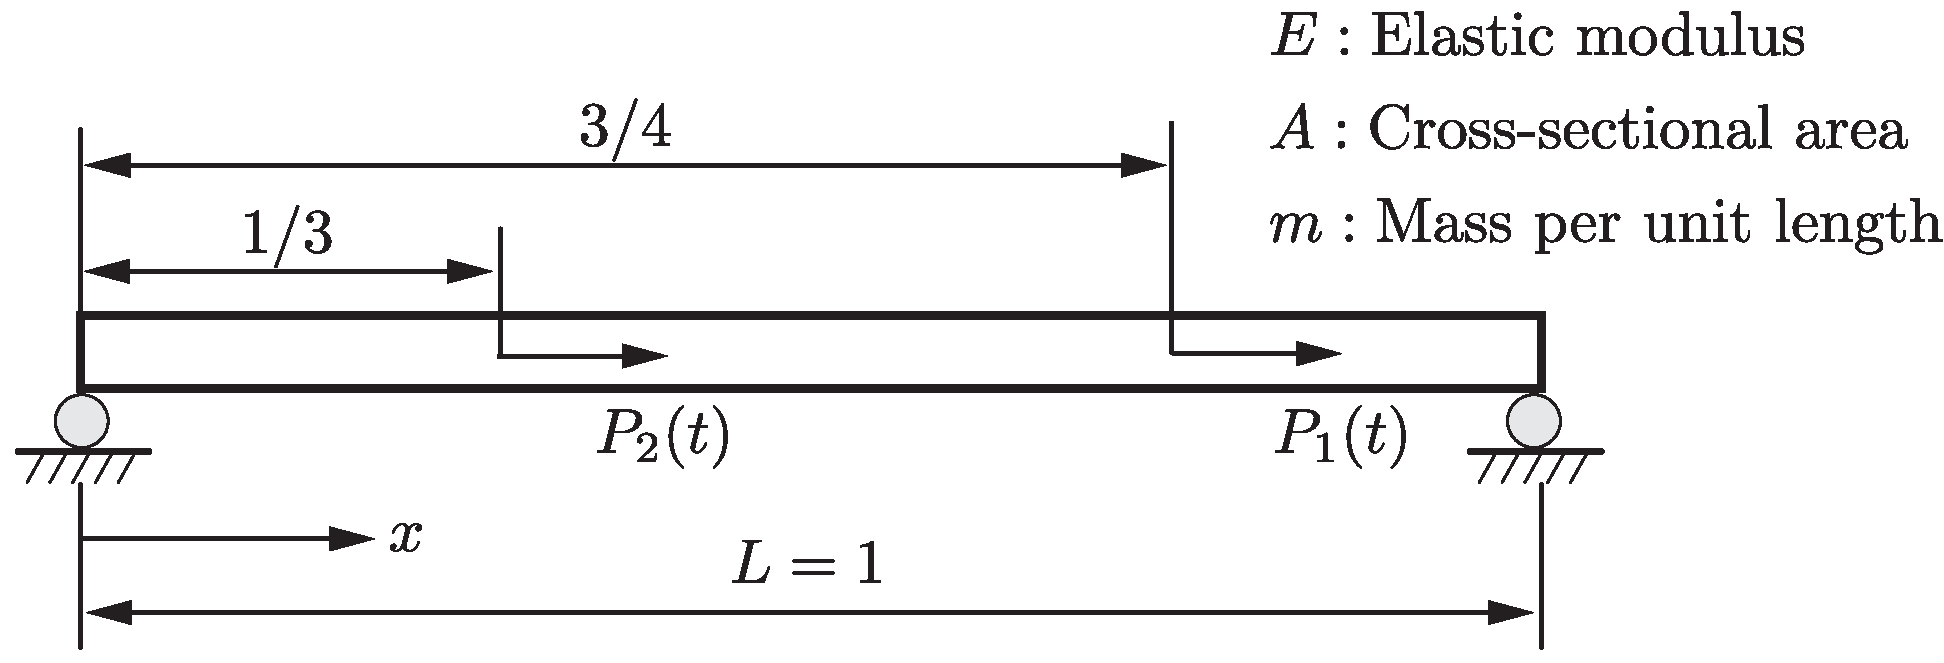
\includegraphics[width=0.7\linewidth]{homework/hw2/assets/hw2_p2.pdf}
\end{figure}

Based on the derivations in class, the governing equation for a rod undergoing axial vibrations is the forced wave equation 
\begin{equation}\label{eqn:hw2_p2_eom}
    m \frac{\partial^2 u}{\partial t^2}(x, t) = E A \frac{\partial^2 u}{\partial x^2}(x, t) + F(x, t)
\end{equation}
where $u(x, t)$ is the axial displacement field, and $m$, $E$, and $A$ are positive constants by virtue of the \emph{uniform rod assumption}. 
Here, $F(x, t)$ consists of two point loads represented as 
\begin{equation}\label{eqn:hw2_p2_force}
    F(x, t) = \left[ \delta\left(x - \frac{3}{4}\right) + 5 \delta\left(x - \frac{1}{3}\right) \right] \left[H(t) - H(t - \pi)\right] \sin t
\end{equation}
where $H(t)$ is the Heaviside function.

We begin the modal analysis by considering the free system ($F(x, t) = 0$), which leads to the classical wave equation 
\begin{equation}
    \frac{\partial^2 u}{\partial t^2}(x, t) = c^2 \frac{\partial^2 u}{\partial x^2}(x, t), ~~~~ c = \sqrt{\frac{EA}{m}},
\end{equation}
where $c$ is the longitudinal wave speed. 
Applying the separable ansatz $u(x, t) = M(x)N(t)$ and the same manipulations in the previous problem, we obtain a system of two linear homogeneous ODEs 
\begin{equation}\label{eqn:hw2_p2_separated}
    \frac{\ddot{N}}{N}(t) = c^2 \frac{M''}{M}(x) = -\omega^2 ~~~~ \Rightarrow  
    \begin{cases}
        M''(x) + {(\omega /c)}^2 M(x) = 0 \\
        \ddot{N}(t) + \omega^2 N(t) = 0
    \end{cases}
\end{equation}
where ``overdots'' denote time derivatives while ``primes'' denote spatial derivatives. 
The placement of $c$ is the spatial ODE ensures dimensional consistency, where the constant $\omega$ is of frequency unit. 

There are two scenarios associated with \cref{eqn:hw2_p2_separated}: $\omega > 0$ (vibration modes) and $\omega = 0$ (rigid / translation mode).
In the case of $\omega = 0$, the only spatial eigenfunction that satisfy the free-boundary conditions is 
\begin{equation}\label{eqn:hw2_p2_M0}
    \boxed{\omega_0 = 0, ~~~~ M_0(x) = C_0 = \sqrt{\frac{1}{mL}}},
\end{equation}
which implies a constant displacement. 
The value of the constant is chosen such that $\int_0^L m {M_0(x)}^2 dx = 1$ which satisfy the mass ortho-normality condition (formulated later). 
For the vibrational modes ($\omega > 0$), the solution is sinusoidal:
\begin{equation}
    M(x) = C \cos\left(\frac{\omega}{c} x\right) + D \sin\left(\frac{\omega}{c} x\right).
\end{equation}
The free-end boundary conditions imply that $EAu_x(0, t) = EAu_x(L, t) = 0$, which under the ansatz leads to $M'(0) = M'(L) = 0$. 
This in turn requires that
\begin{equation}
    D = 0, ~~~~ \sin\left(\frac{\omega}{c}L\right) = 0 ~~ \Rightarrow ~~ \boxed{\omega_n = \frac{c}{L} n\pi = \sqrt{\frac{EA}{mL^2}} n\pi, ~~~~ n = 1, 2, 3, \ldots}
\end{equation}
where $\omega_1 < \omega_2 < \ldots$ are the countable-infinite number of natural frequencies.
The corresponding eigenfunctions are
\begin{equation}\label{eqn:hw2_p2_eigenfunctions}
    \boxed{M_n(x) = C_n \cos\left( n\pi \frac{x}{L}\right), ~~~~ C_n = {\left[m\int_0^L \cos^2\left(n\pi \frac{x}{L} \right) ~dx\right]}^{-\frac{1}{2}} = \sqrt{\frac{2}{mL}}, ~~~~ n = 1, 2, 3, \ldots}
\end{equation}
where $C_n$ is defined such that the eigenfunctions are orthonormal with respect to mass $m$: 
\begin{equation}\label{eqn:hw2_p2_orthonormality}
    \int_0^L m M_i(x)M_j(x) ~dx = \delta_{ij}, ~~~~ i, j = 0, 1, 2, 3, \ldots
\end{equation}
Note that the orthogonality is naturally satisfied as the sinusoidal eigenfunctions are orthogonal functions over the domain $[0, L]$, and the rigid body mode \cref{eqn:hw2_p2_M0} is also naturally encompassed in this condition.

The separable ansatz is now expressed as a linear combination $u(x, t) = \sum_{i=0}^\infty M_i(x) N_i(t)$, which is substituted back into the forced equation of motion \cref{eqn:hw2_p2_eom} to obtain 
\begin{equation}
\begin{aligned}
    m \sum_{i=0}^\infty \ddot{N}_i(t) M_i(x) &= E A \sum_{i=0}^\infty N_i(t) M''_i(x) + F(x, t) \\
    &= -m \sum_{i=0}^\infty \omega_i^2 N_i(t) M_i(x) + F(x, t),
\end{aligned}
\end{equation}
where the second step follows from \cref{eqn:hw2_p2_separated}.
Here, we have employed the same temporal dependent variable $N_j(t)$ as before, but the same ODE in \cref{eqn:hw2_p2_separated} is no longer satisfied as we are now considering the forced system.
By taking the inner product with $M_j(x)$ (for a fixed $j = 0, 1, 2, 3, \ldots$) over the spatial domain $[0, L]$ and leveraging the ortho-normality condition \cref{eqn:hw2_p2_orthonormality}, we obtain the temporal ODE for the $j$-th mode:
\begin{equation}\label{eqn:hw2_p2_Nj_ode}
\begin{aligned}
    \ddot{N}_0(t) &= \int_0^L M_0(x) F(x, t) ~dx \\
    &= \frac{6}{\sqrt{mL}} \left[H(t) - H(t - \pi)\right] \sin t \\
    \ddot{N}_j(t) + \omega_j^2 N_j(t) &= \int_0^L M_j(x) F(x, t) ~dx, ~~~~ j = 1, 2, 3, \ldots \\ 
    &= \sqrt{\frac{2}{mL}} \left[ \cos\left( \frac{3}{4}j\pi \right) + 5\cos\left( \frac{1}{3}j\pi \right) \right] \left[H(t) - H(t - \pi)\right] \sin t
\end{aligned}
\end{equation}
where we have substituted in \cref{eqn:hw2_p2_force,eqn:hw2_p2_eigenfunctions}. 

Before proceeding, we assume the following initial conditions 
\begin{equation}
    u(x, 0) = \sum_{i=0}^\infty M_i(x) N_i(0) = g(x), ~~~~ \frac{\partial u}{\partial t}(x, 0) = \sum_{i=0}^\infty M_i(x) \dot{N}_i(0) = h(x)
\end{equation}
Taking their $m$-inner products with $M_j(x)$ for some $j = 0, 1, 2, \ldots$ yields the initial conditions for $N_j(t)$:
\begin{equation}\label{eqn:hw2_p2_Nj_bc}
    N_j(0) = \int_0^L m M_j(x) g(x) ~dx, ~~~~ \dot{N}_j(0) = \int_0^L m M_j(x) h(x) ~dx
\end{equation} 
Furthermore, due to the abrupt change in the forcing function at $t = \pi$, we opt to solve for the solution on two intervals: $t \in [0, \pi]$ and $t \in (\pi, \infty)$. 
The piecewise solutions at $t = \pi$ must satisfy displacement and velocity continuity, namely 
\begin{equation}
    N_j^{(1)}(\pi) = N_j^{(2)}(\pi), ~~~~ \dot{N}_j^{(1)}(\pi) = \dot{N}_j^{(2)}(\pi), ~~~~ N_j(t) = H(t)N_j^{(1)}(t) + H(t - \pi) \left[N_j^{(2)}(t) - N_j^{(1)}(t) \right]
\end{equation}
where the superscripts denote the two intervals. 

We now solve the countable-infinite number of modal oscillators \cref{eqn:hw2_p2_Nj_ode} subjected to the boundary conditions \cref{eqn:hw2_p2_Nj_bc}. 
For conciseness, some of the more strenuous arithmetics are omitted here. 
The result reads 
\begin{equation}
\begin{aligned}
    N_0^{(1)}(t) &= N_0(0) + \left[\dot{N}_0(0) + \frac{6}{\sqrt{mL}}\right]t - \frac{6}{\sqrt{mL}}\sin t, \\
    N_0^{(2)}(t) &= \left[\dot{N}_0(0) + \frac{12}{\sqrt{mL}}\right] t + N_0(0) - \frac{6\pi}{\sqrt{mL}}, \\
    N_j^{(1)}(t) &= N_j(0) \cos\omega_j t + \frac{1}{\omega_j}\dot{N}_j(0)\sin\omega_j t \\
    &~~~+ \frac{1}{\omega_j^2 - 1}\sqrt{\frac{2}{mL}} \left[ \cos\left( \frac{3}{4}j\pi \right) + 5\cos\left( \frac{1}{3}j\pi \right) \right] \left(\sin t - \frac{1}{\omega_j}\sin\omega_j t\right), \\
    N_j^{(2)}(t) &= N_j(0) \cos\omega_j t + \frac{1}{\omega_j} \left\{ \dot{N}_j(0) - \frac{1}{\omega_j^2 - 1}\sqrt{\frac{2}{mL}} \left[ \cos\left( \frac{3}{4}j\pi \right) + 5\cos\left( \frac{1}{3}j\pi \right) \right] \right\} \sin\omega_j t, 
\end{aligned}
\end{equation}
where $j = 1, 2, 3, \ldots$ and $i = 0, 1, 2, 3, \ldots$. 
Note that the above solutions are valid for the \emph{non-resonant cases}, i.e. $\omega_j \neq 1$. 
In the case of resonance (without loss of generality, assume $\omega_j = 1$), we have instead 
\begin{equation}
\begin{aligned}
    N_j^{(1)}(t) &= N_j(0) \cos t + \dot{N}_j(0) \sin t + \frac{1}{\sqrt{2mL}} \left[ \cos\left( \frac{3}{4}j\pi \right) + 5\cos\left( \frac{1}{3}j\pi \right) \right] (\sin t - t \cos t), \\
    N_j^{(2)}(t) &= \left\{ N_j(0) - \frac{\pi}{\sqrt{2mL}} \left[ \cos\left( \frac{3}{4}j\pi \right) + 5\cos\left( \frac{1}{3}j\pi \right) \right] \right\}  \cos t + \dot{N}_j(0) \sin t.
\end{aligned}
\end{equation}
Finally, the solution is written as $\boxed{u(x, t) = \sum_{i=0}^\infty M_i(x) N_i(t)}$.

\begin{problem}
\begin{wrapfigure}{r}{0.3\textwidth}
    \vspace{-16pt}
    \centering
    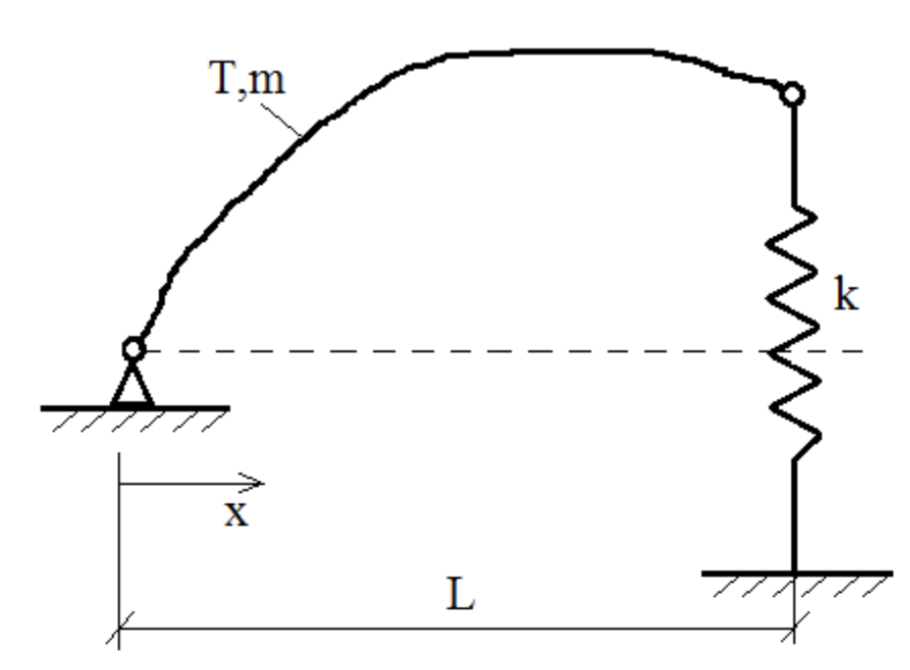
\includegraphics[width=0.9\linewidth]{homework/hw2/assets/hw2_p3.png}
\end{wrapfigure}
\textbf{3 (50 pts).} Compute the normal vibration modes of the uniform elastic string with fixed boundary condition at its left end and a transverse linear spring of constant $k$ at its right end. 
Mass-orthonormalize the derived eigenfunctions. 
Assume that the spring can only deform in the vertical direction. 
Show that in the limit $k\rightarrow 0$ the modes approach those of the fixed-free string, whereas for $k\rightarrow \infty$ they approach the fixed-fixed string.
\end{problem}

Let the vertical deflection of the string be $u(x, t): [0,L]\times[0, \infty] \mapsto \mathbb{R}$. 
The governing equation of this free system, same as Problem 1, 
\begin{equation}
    m \frac{\partial^2 u}{\partial t^2}(x, t) = \frac{\partial }{\partial x} \left[T \frac{\partial u}{\partial x}(x, t)\right]
\end{equation}
where we the mass per unit length $m$ and tension $T$ to be \emph{constant}. 
The boundary conditions are 
\begin{equation}\label{eqn:hw2_p3_bc}
    u(0,t) = 0, ~~~~ T \frac{\partial u}{\partial x}(L, t) + k u(L, t) = 0
\end{equation}
where the second BC can be derived by integrating $mu_{tt} = Tu_{xx} + ku\delta(x-L)$ over a small interval $[L-\epsilon, L+\epsilon]$ and then taking the limit $\epsilon \rightarrow 0$: 
\begin{equation}
\begin{aligned}
    0 &= \lim_{\epsilon \rightarrow 0} \int_{L-\epsilon}^{L+\epsilon} \left[m \frac{\partial^2 u}{\partial t^2} - T \frac{\partial^2 u}{\partial x^2} + ku\delta(x-L)\right] dx \\
    &= \lim_{\epsilon\rightarrow 0} {\left[ -T \frac{\partial u}{\partial x} + \order{\epsilon} \right]}_{L-\epsilon}^{L+\epsilon} + ku(L, t) \\
    &= T \frac{\partial u}{\partial x}(L, t) + k u(L, t).
\end{aligned}
\end{equation}
The integral of the inertial term is of order $\order{\epsilon}$ and thus vanishes in the limit. 

We note that the governing equation here is also the classical wave equation, same as in Problem 2 but with $c = \sqrt{T / m}$. 
However, the boundary conditions are different, which requires a different set of eigenvalues and eigenfunctions.
Following the same procedure as in Problem 2, we create the separable ansatz 
\begin{equation}\label{eqn:hw2_p3_ansatz}
    u(x, t) = M(x) N(t)
\end{equation}
which leads to the system of ODEs:
\begin{equation}\label{eqn:hw2_p3_separated}
    M''(x) + \frac{\omega^2}{c^2} M(x) = 0, ~~~~ \ddot{N}(t) + \omega^2 N(t) = 0
\end{equation}
and arrives at the general solution for the spatial modes:
\begin{equation}\label{eqn:hw2_p3_M_general}
    M(x) = A \cos\left(\frac{\omega}{c} x\right) + B \sin\left(\frac{\omega}{c} x\right).
\end{equation}
Note that the rigid body modes do no appear here as the left boundary is fixed. 
Substituting the ansatz \cref{eqn:hw2_p3_ansatz} into the boundary conditions \cref{eqn:hw2_p3_bc} yields
\begin{equation}\label{eqn:hw2_p3_bc_spatial}
    M(0) = 0, ~~~~ T M'(L) + k M(L) = 0
\end{equation}
which, in conjunction with \cref{eqn:hw2_p3_M_general}, leads to 
\begin{equation}
    A = 0, ~~~~ B \neq 0, ~~~~ T \frac{\omega}{c} \cos\left(\frac{\omega}{c} L\right) + k \sin\left(\frac{\omega}{c} L\right) = 0 
\end{equation}
where $\omega$ cannot be solved for in closed form. 
A more straightforward form of the eigenvalue equation is obtained by defining a non-dimensional variable $\eta_n$ such that 
\begin{equation}\label{eqn:hw2_p3_eigenvalue_eqn}
    \tan\eta_n = -\frac{T}{kL} \eta_n, ~~~~ \eta_n := \frac{\omega_n L}{c} > 0, ~~~~ n = 1, 2, 3, \ldots,
\end{equation}
which leads to a countable-infinite number of eigenvalues due to the infinite branches of the tangent functions. 
The corresponding eigenfunctions are
\begin{equation}\label{eqn:hw2_p3_eigenfunctions}
    \boxed{M_n(x) = B_n \sin\left(\frac{\omega_n}{c} x\right), ~~~~ n = 1, 2, 3, \ldots},
\end{equation}
where $B_n$ is chosen to satisfy the mass ortho-normality condition:
\begin{equation}
    B_n = {\left[m\int_0^L \sin^2\left(\frac{\omega_n}{c} x\right) dx \right]}^{-\frac{1}{2}} = { \left\{ \frac{mL}{2} \left[ 1 - \frac{\sin (2\eta_n)}{2\eta_n} \right] \right\} }^{-\frac{1}{2}} 
\end{equation}
The mass-orthogonality of the eigenfunctions is derived from \cref{eqn:hw2_p3_separated} as 
\begin{equation}\label{eqn:hw2_p3_orthogonal_proof}
\begin{aligned}
    0 &= \int_0^L \left[ T M_i''(x) + \omega_i^2 m M_i(x) \right] M_j(x) dx \\
    &= {\left[ T M_i'(x) M_j(x) \right]}_0^L - \int_0^L T M_i'(x) M_j'(x) dx + \omega_i^2  \int_0^L m M_i(x) M_j(x) dx \\
    & = {\left[ T M_i'(x) M_j(x) - T M_i(x)M_j'(x)\right]}_0^L + \int_0^L T M_i(x) M_j''(x) dx + \omega_i^2  \int_0^L m M_i(x) M_j(x) dx \\
    &= -kM_i(L)M_j(L) + kM_i(L)M_j(L) - \int_0^L \left[\omega_j^2 m M_j(x)\right] M_i(x) dx + \omega_i^2\int_0^L m M_i(x) M_j(x) dx \\ 
    &= (\omega_i^2 - \omega_j^2) \int_0^L m M_i(x) M_j(x) dx
\end{aligned}
\end{equation}
for some $j = 1, 2, 3, \ldots$ where we have integrated by parts twice and applied the boundary conditions \cref{eqn:hw2_p3_bc_spatial} to eliminate the boundary terms. 
Note that the spring stiffness does not appear here, consistent with conclusions from the lecture. 
It shows that for $i \neq j$, the eigenfunctions \cref{eqn:hw2_p3_eigenfunctions} are mass-orthogonal, and $B_n$ is selected such that
\begin{equation}\label{eqn:hw2_p3_orthonormality}
    \int_0^L m M_i(x) M_j(x) dx = \delta_{ij}.
\end{equation}
This concludes the derivation for the spatial eigenpairs $\{\omega_i, M_i(x; \omega_i)\}$. 
Due to the lack of external forcing, the temporal ODE from \cref{eqn:hw2_p3_separated} still holds:
\begin{equation}
    \ddot{N}_i(t) + \omega_i^2 N_i(t) = 0, ~~ \Rightarrow ~~ N_i(t) = C_i \cos\omega_i t + D_i \sin\omega_i t.
\end{equation}
Assume the initial conditions to be 
\begin{equation}
    u(x, 0) = \sum_{i=1}^\infty M_i(x) N_i(0)= g(x), ~~~~ \frac{\partial u}{\partial t}(x, 0) = \sum_{i=1}^\infty M_i(x) \dot{N}_i(0) = h(x).
\end{equation}
Computing the $m$-inner product of the initial conditions with $M_j(x)$ while leveraging the mass ortho-normality condition \cref{eqn:hw2_p3_orthonormality} leads to 
\begin{equation}
    N_j(0) = \int_0^L m B_j \sin \left(\eta_j \frac{x}{L} \right)g(x) ~dx, ~~~~ \dot{N}_j(0) = \int_0^L m B_j \sin \left(\eta_j \frac{x}{L} \right) h(x) ~dx.
\end{equation}
which uniquely determines the unknown coefficients $C_i$ and $D_i$ for each mode as 
\begin{equation}
    C_i = N_i(0), ~~~~ D_i = \frac{\dot{N}_i(0)}{\omega_i}.
\end{equation}
The full solution then reads 
\begin{equation}\label{eqn:hw2_p3_soln}
    \boxed{u(x, t) = \sum_{i=1}^\infty M_i(x) N_i(x) = \sum_{i=1}^\infty B_i \sin\left(\frac{\omega_i}{c} x\right)\left[ N_i(0) \cos\omega_i t + \frac{\dot{N}_i(0)}{\omega_i} \sin\omega_i t \right]}.
\end{equation}
where the spring stiffness $k$ is only used to determine the eigenvalues $\omega_i$. 

We now discuss the solution behavior in the limits $k \rightarrow 0$ and $k \rightarrow \infty$. 
First, note that if the boundary condition at $x = L$ is modified to a fixed or free boundary, the solution would still be of the same form as \cref{eqn:hw2_p3_soln}, but with different eigenvalues $\omega_n$ (or $\eta_n := \omega_n L / c$):
\begin{subequations}
\begin{align}
    \label{eqn:hw2_p3_fixed_fixed}(\textrm{fixed-fixed}) ~~~~& \eta_n = n\pi, && n = 1, 2, 3, \ldots, \\
    \label{eqn:hw2_p3_fixed_free}(\textrm{fixed-free}) ~~~~& \eta_n = \left(n - \frac{1}{2}\right)\pi, && n = 1, 2, 3, \ldots.
\end{align}
\end{subequations}
The same eigenvalues can be obtained by examining \cref{eqn:hw2_p3_eigenvalue_eqn} in the limits $k \rightarrow 0$ and $k \rightarrow \infty$:
\begin{subequations}
\begin{align}
    \tan\eta_n &= \lim_{k\rightarrow \infty}\left(- \frac{T}{kL}\eta_n\right) = 0, && \Rightarrow ~~ \eta_n \rightarrow n\pi, & n = 1, 2, 3, \ldots, \\
    \tan\eta_n &= \lim_{k\rightarrow 0^+}\left(- \frac{T}{kL}\eta_n\right) = -\infty, && \Rightarrow ~~ \eta_n \rightarrow \left(n - \frac{1}{2}\right)\pi, & n = 1, 2, 3, \ldots,
\end{align}
\end{subequations}
which is consistent with \cref{eqn:hw2_p3_fixed_fixed,eqn:hw2_p3_fixed_free}, respectively.
Therefore, when $k\rightarrow \infty$, the system approaches the behavior of a fixed-fixed string, while for $k\rightarrow 0$, it approaches that of a fixed-free string. 

This result can also be argued graphically (\cref{fig:hw2_p3_eval_eqn}) by finding the intersections of both sides of \cref{eqn:hw2_p3_eigenvalue_eqn}. 
By letting $k\rightarrow \infty$, the dash-dot line approaches the horizontal axis, resulting in the roots approaching $n\pi$ (fixed-fixed). 
Conversely, as $k\rightarrow 0$, the dash-dot line approaches the vertical axis, which intersect each tangent branch at negative infinity, corresponding to $\eta_n = (n-0.5)\pi$ (fixed-free). 
\begin{figure}[!ht]
    \centering
    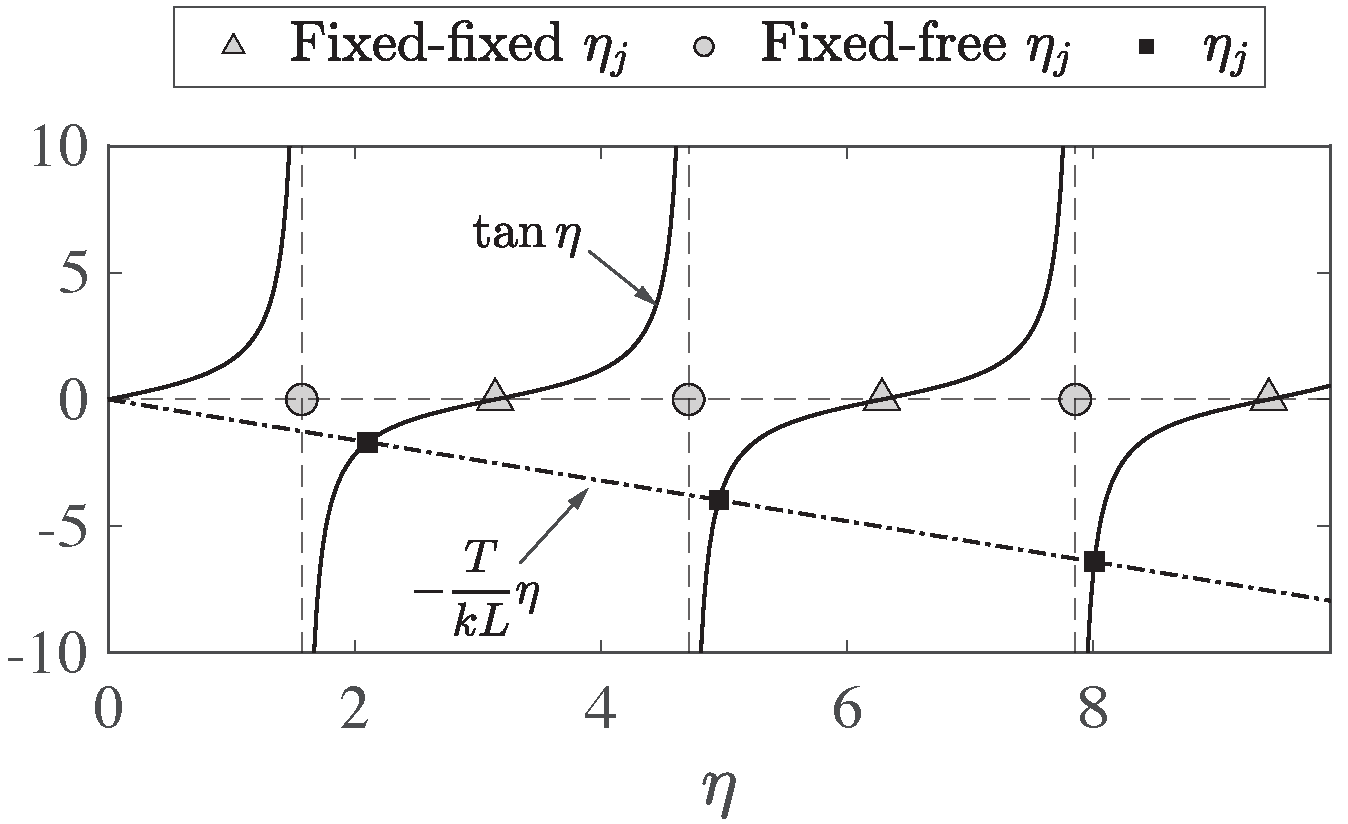
\includegraphics[width=0.6\textwidth]{homework/hw2/assets/hw2_p3_eval_eqn.pdf}
    \caption{Graphical representation to the solution of \cref{eqn:hw2_p3_eigenvalue_eqn}. The eigenvalues (or rather, $\eta_i$) are obtained as the $\eta$-values of intersections between the tangent function and the linear function $-T\eta / kL$. The triangles and circles represent the eigenvalues for the fixed-fixed and fixed-free boundary conditions, respectively.}
    \label{fig:hw2_p3_eval_eqn}
\end{figure}


\begin{problem}
\textbf{4 (50 pts).} Consider the second-order linear differential equation:
\begin{equation}
\begin{aligned}
    &\ddot{x}(t) + p(t) \dot{x}(t) + q(t) x(t) = f(t) \\
    &x(0) = X, ~\dot{x}(0) = V
\end{aligned}
\end{equation}
Show that if one homogeneous solution is known, then you can compute the complete solution of the initial value problem (that is, you can compute a second linearly independent homogeneous solution and a particular integral).
\end{problem}

First, consider the homogeneous equation (i.e. $f(t) = 0$). 
Assume that we know one solution $x_1(t)$ such that 
\begin{equation}
    \ddot{x}_1(t) + p(t) \dot{x}_1(t) + q(t) x_1(t) = 0.
\end{equation}
For now, we \emph{assume $x_1(t) \neq 0, \forall t \geq 0$}, which avoids some singularities. 
Two common approaches can be used to find the other homogeneous solution $x_2(t)$, both of which listed below. 
\begin{enumerate}[(i)]
\item {
    \emph{Wronskian}. We require that the two solutions are linearly independent, which dictates that $a_1 x_1(t) + a_2 x_2(t) = 0$ holds only when $a_1 = a_2 = 0$. 
    Taking derivatives once, this leads to a linearly system 
    \begin{equation}
        \begin{bmatrix}
            x_1(t) & x_2(t) \\
            \dot{x}_1(t) & \dot{x}_2(t)
        \end{bmatrix} \begin{bmatrix}
            a_1 \\ a_2
        \end{bmatrix} = \bv{0}, ~~~~ \iff ~~~~ a_1 = a_2 = 0.
    \end{equation}
    which implies the determinant, formally known as the Wronskian determinant, must be non-zero:
    \begin{equation}
        W(t) := W[x_1, x_2](t) \equiv \det \begin{bmatrix}
            x_1(t) & x_2(t) \\
            \dot{x}_1(t) & \dot{x}_2(t)
        \end{bmatrix} = x_1(t) \dot{x}_2(t) - \dot{x}_1(t) x_2(t) \neq 0.
    \end{equation}
    Furthermore, we may take the derivative of the Wronskian to find (Abel's Theorem)
    \begin{equation}
    \begin{aligned}
        \frac{dW}{dt}(t) &= x_1(t) \ddot{x}_2(t) - \ddot{x}_1(t) x_2(t) \\
        &= x_1(t) \left[-p(t) \dot{x}_2(t) - q(t) x_2(t) \right] - \left[-p(t) \dot{x}_1(t) - q(t) x_1(t) \right]x_2(t) \\
        &= -p(t) W(t) \\
        \Rightarrow ~~ \Aboxed{W(t) &= W(0) e^{-\int_0^t p(\tau) d\tau}}.
    \end{aligned}
    \end{equation}
    where $W(0) \neq 0$. 
    With $x_1(t) \neq 0$ known, we can find $x_2(t)$ by 
    \begin{equation}
        \int_0^t \frac{W(\tau)}{{x_1(\tau)}^2} d\tau = \int_0^t \frac{x_1(\tau) \dot{x}_2(\tau) - \dot{x}_1(\tau) x_2(\tau)}{{x_1(\tau)}^2} d\tau = \frac{x_2(t)}{x_1(t)} + \textrm{const.}
    \end{equation}
    where the trailing constant can be ignored as it merely represents adding a $x_1(t)$ component to $x_2(t)$. 
    Furthermore, the Wronskian contains an unknown constant $W(0)$ which can be left as any non-zero value at the moment. 
    Rearranging yields 
    \begin{equation}\label{eqn:hw2_p4_x2_wronskian}
        \boxed{x_2(t) = x_1(t) \int_0^t \frac{W(\tau)}{{x_1(\tau)}^2} d\tau}.
    \end{equation}
}
\item {
    \emph{Reduction of order}. We create an ansatz $x_2(t) = u(t)x_1(t)$ where $u_1(t)$ is twice differentiable for $t > 0$. 
    If $x_2(t)$ satisfies the ODE, we require that 
    \begin{equation}
    \begin{aligned}
        0 & = \ddot{x}_2(t) + p(t) \dot{x}_2(t) + q(t) x_2(t) \\
        &= \ddot{u}x_1 + 2\dot{u}\dot{x}_1 + u \ddot{x}_1 + p\dot{u}x_1 + pu\dot{x}_1 + q ux_1 \\
        &= x_1\ddot{u} + (2\dot{x}_1 + px_1) \dot{u}\\
    \end{aligned}
    \end{equation}
    where $\dot{u}$ satisfy a first-order separable ODE whose solution reads 
    \begin{equation}
        \dot{u}(t) = C {x_1(t)}^{-2} e^{-\int_0^t p(\tau) d\tau}
    \end{equation}
    Integrating again and setting $C = 1$ yields 
    \begin{equation}
        \boxed{x_2(t) = u(t) x_1(t) = x_1(t) \int_0^t \frac{e^{-\int_0^\tau p(\xi) d\xi}}{x_1^2(\tau)} d\tau}.
    \end{equation}
    which is identical to \cref{eqn:hw2_p4_x2_wronskian} up to a multiplicative factor. 
}
\end{enumerate}

The two methods above are equivalent and leads to the same solution. 
They are derived based on the assumption that $x_1(t) \neq 0$ for all $t \geq 0$.
If $x_1(t) = 0$ for some $t$ and the singularity cannot be regularized, then a more sophisticated approach may be required. 

Once $x_1(t)$ and $x_2(t)$ are found, the inhomogeneous solution can be found by \emph{variation of parameters}. 
The ansatz is $x_s(t) = v_1(t) x_1(t) + v_2(t) x_2(t)$ and 
\begin{equation}
\begin{aligned}
    \dot{x}_s(t) &= v_1(t) \dot{x}_1(t) + v_2(t) \dot{x}_2(t) + \underbrace{\dot{v}_1(t) x_1(t) + \dot{v}_2(t) x_2(t)}_{\textrm{assume} = 0} \\
    \ddot{x}_s(t) &= v_1(t) \ddot{x}_1(t) + v_2(t) \ddot{x}_2(t) + \dot{v}_1(t) \dot{x}_1(t) + \dot{v}_2(t) \dot{x}_2(t).
\end{aligned}
\end{equation}
If $x_s(t)$ satisfies the inhomogeneous ODE $\ddot{x}_s(t) + p(t)\dot{x}_s(t) + q(t)x_s(t) = f(t)$, then the following system must be satisfied:
\begin{equation}
    \begin{bmatrix}
        x_1(t) & x_2(t) \\
        \dot{x}_1(t) & \dot{x}_2(t)
    \end{bmatrix} \begin{bmatrix}
        \dot{v}_1(t) \\ \dot{v}_2(t)
    \end{bmatrix} = \begin{bmatrix}
        0 \\ f(t)
    \end{bmatrix}
\end{equation}
where the imposing matrix is the \emph{Wronskian matrix} denoted as $\bt{W}(t)$. 
After inverting the system, the inhomogeneous solution then reads
\begin{equation}
    \boxed{x_s(t) = \begin{bmatrix}
        x_1(t) \\ x_2(t) 
    \end{bmatrix}^T \int_0^t \bt{W}^{-1}(\tau) \begin{bmatrix}
        0 \\ f(\tau)
    \end{bmatrix} d\tau}.
\end{equation}
Collecting the terms, the general solution is 
\begin{equation}
    x(t) = c_1 x_1(t) + c_2 x_2(t) + x_s(t)
\end{equation}
where $c_1$ and $c_2$ are determined by the initial conditions $x(0) = X$ and $\dot{x}(0) = V$.

\begin{problem}
\textbf{5 (100 pts).} Consider the following rod in axial vibrations with an oscillator attached to it. 
\begin{enumerate}[(i)]
    \item Compute the normal modes (natural frequencies and eigenfunctions) and derive the ortho-normality conditions satisfied by the eigenfunctions.
    \item Solve graphically the frequency equation to show that this system has a countably infinite discrete set of natural frequencies. 
    Is it possible to have repeated natural frequencies?
    \item What happens in the limits $K\rightarrow \infty$, $K\rightarrow 0$, or $M\rightarrow \infty$?
    \item Discuss how you can user modal analysis to compute the free response of the rod to initial conditions:
    \begin{equation}
        u(x, 0) = U(x), ~~ u_t(x, 0) = V(x), ~~ y(0) = \dot{y}(0) = 0.
    \end{equation}
\end{enumerate}
\end{problem}

\begin{figure}[!ht]
    \centering
    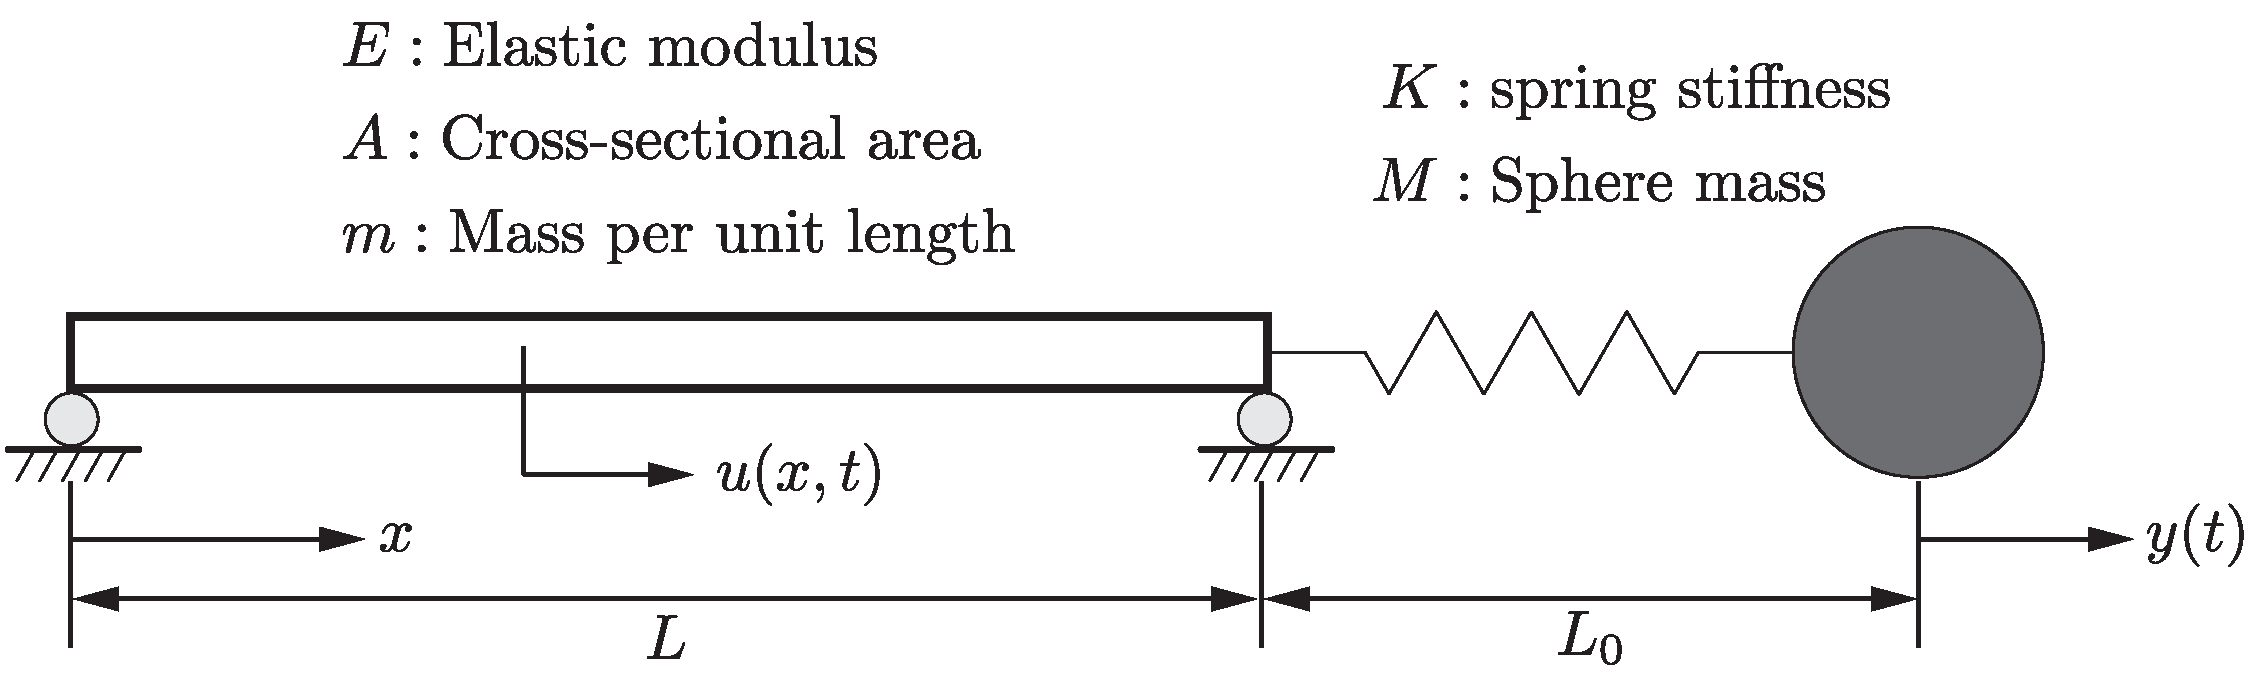
\includegraphics[width=0.8\textwidth]{homework/hw2/assets/hw2_p5.pdf}
\end{figure}


We assume the \emph{left end of the rod is free}, $L_0$ is the rest length of the spring, and $y(t)$ is counted with respect to $x = L + L_0$. 
Parameters $m$, $EA$, $K$, and $M$ are assumed to be constant. 

\begin{enumerate}[(i)]
\item { % 5(i)
    The equations of motion of this system can be written as 
    \begin{subequations}
    \begin{align}
        \label{eqn:hw3_p5_eom_rod} m \frac{\partial^2 u}{\partial t^2}(x, t) &= EA \frac{\partial^2 u}{\partial x^2}(x, t) + K \left[ y(t) - u(L, t)\right] \delta(x - L) \\
        \label{eqn:hw3_p5_eom_mass} M \frac{d^2y}{dt^2} &= -K \left[ y(t) - u(L, t)\right]
    \end{align}
    \end{subequations}
    wherein for the continuous rod (\cref{eqn:hw3_p5_eom_rod}) the spring-mass boundary is formulated as an external force via the Dirac delta function.
    To make modal analysis tractable, we treat the two displacement fields $u(x, t)$ and $y(t)$ separately, with the former absolved in the boundary condition and the latter acting as the forcing term. 
    The two major steps involved in the modal analysis are outlined as follows:
    \begin{enumerate}[(a)]
        \item {
            Consider the unforced system with free-spring boundary conditions
            \begin{equation}
            \begin{gathered}
                m u_{tt}(x, t) = EA u_{xx}(x, t) \\
                u_x(0, t) = 0, ~~~~ EAu_x(L, t) + Ku(L, t) = 0
            \end{gathered}
            \end{equation}
            and proceed with the separable ansatz $u(x, t) = \varphi(x)\eta(t)$ to find the spatial modal eigenpairs.
        }
        \item {
            After obtaining the spatial modes, substitute $u(x, t) = \sum_{i=0}^\infty \varphi_i(x)\eta_i(t)$ back into the forced system 
            \begin{equation}
            \begin{aligned}
                m u_{tt}(x, t) &= EA u_{xx}(x, t) + Ky(t)\delta(x - L) \\
                M \ddot{y}(t) &= -K \left[ y(t) - u(L, t)\right]
            \end{aligned}
            \end{equation}
            with initial conditions to find the temporal modes $\eta_i(t)$.
        }
    \end{enumerate}

    We start by resolving step (a). 
    Let $u(x, t) = \varphi(x)\eta(t)$ and the spatial ODE (with boundary conditions), as shown many times before, reads 
    \begin{equation}
    \begin{gathered}
        \varphi''(x) + \frac{\omega^2}{c^2}\varphi(x) = 0, ~~~~ c = \sqrt{\frac{EA}{m}} \\
        \varphi'(0) = 0, ~~~~ EA\varphi'(L) + K\varphi(L) = 0.
    \end{gathered}
    \end{equation}
    Note that the rigid body mode $\omega = 0$ is not permitted (leads to trivial $\varphi = 0$), despite the system as a whole is not constrained by Dirichlet boundaries. 
    Hence, the general solution is sinusoidal:
    \begin{equation}
        \varphi(x) = C \cos\left(\frac{\omega}{c} x\right) + D \sin\left(\frac{\omega}{c} x\right),
    \end{equation}
    and to satisfy the boundary conditions,
    \begin{equation}\label{eqn:hw3_p5_eigenvalue_eqn}
        D = 0, ~~~~ -EA\frac{\omega}{c} \sin\left(\frac{\omega}{c} L\right) + K \cos\left(\frac{\omega}{c} L\right) = 0.
    \end{equation}
    which must be solved through graphical or numerical methods to find a countable-infinite number of eigenvalues (solved in (ii)). 
    With $\omega_i$ determined, the spatial eigenfunctions are then 
    \begin{equation}
        \boxed{\varphi_i(x) = C_i \cos\left(\frac{\omega_i}{c} x\right)},  
    \end{equation}
    which are readily shown to be mass-orthogonal (see Problem 3 \cref{eqn:hw2_p3_orthogonal_proof} for a similar proof).
    To satisfy the mass ortho-normality condition $\int_0^L m\varphi_i(x) \varphi_j(x) dx = \delta_{ij}$, we require that 
    \begin{equation}
    \begin{aligned}
        C_i &= {\left[m\int_0^L \cos^2\left(\frac{\omega_i}{c} x\right) dx \right]}^{-\frac{1}{2}} \\
        &= { \left\{ \frac{m}{2}\int_0^L \left[1 + \cos\left(2\frac{\omega_i}{c} x\right) \right] dx \right\} }^{-\frac{1}{2}} \\
        &= { \left\{ \frac{mL}{2} \left[ 1 + \frac{\sin (2\rho_i)}{2\rho_i} \right] \right\} }^{-\frac{1}{2}} 
    \end{aligned}
    \end{equation}
    where $\rho_i := \omega_i L / c$ are the non-dimensionalized natural frequencies (see (ii)). 
}
\item { % 5(ii)
    The implicit equation for $\omega_i$ in \cref{eqn:hw3_p5_eigenvalue_eqn} can be reformulated as 
    \begin{equation}\label{eqn:hw2_p5_eval_eqn}
        \boxed{\tan \rho = \frac{KL}{EA} \frac{1}{\rho}, ~~~~ \rho := \frac{\omega L}{c} > 0}.
    \end{equation}
    The eigenvalues (by proxy of $\rho$) are obtained as the intersections of the tangent and hyperbolic functions, as shown in \cref{fig:hw2_p5_eval_eqn}.
    As the hyperbolic function extends to $\rho \rightarrow \infty$ and the tangent function has an infinite number of branches, the system has a \emph{countably infinite number of natural frequencies}.
    Specifically, there exists a unique intersection $\rho_i$ corresponding to each branch of the tangent function, so there is \emph{no possibility of repeating natural frequencies} ($\rho_n \in ((n-1)\pi, (n-0.5)\pi), ~n=1, 2, 3,\ldots$). 
    \begin{figure}[!ht]
        \centering
        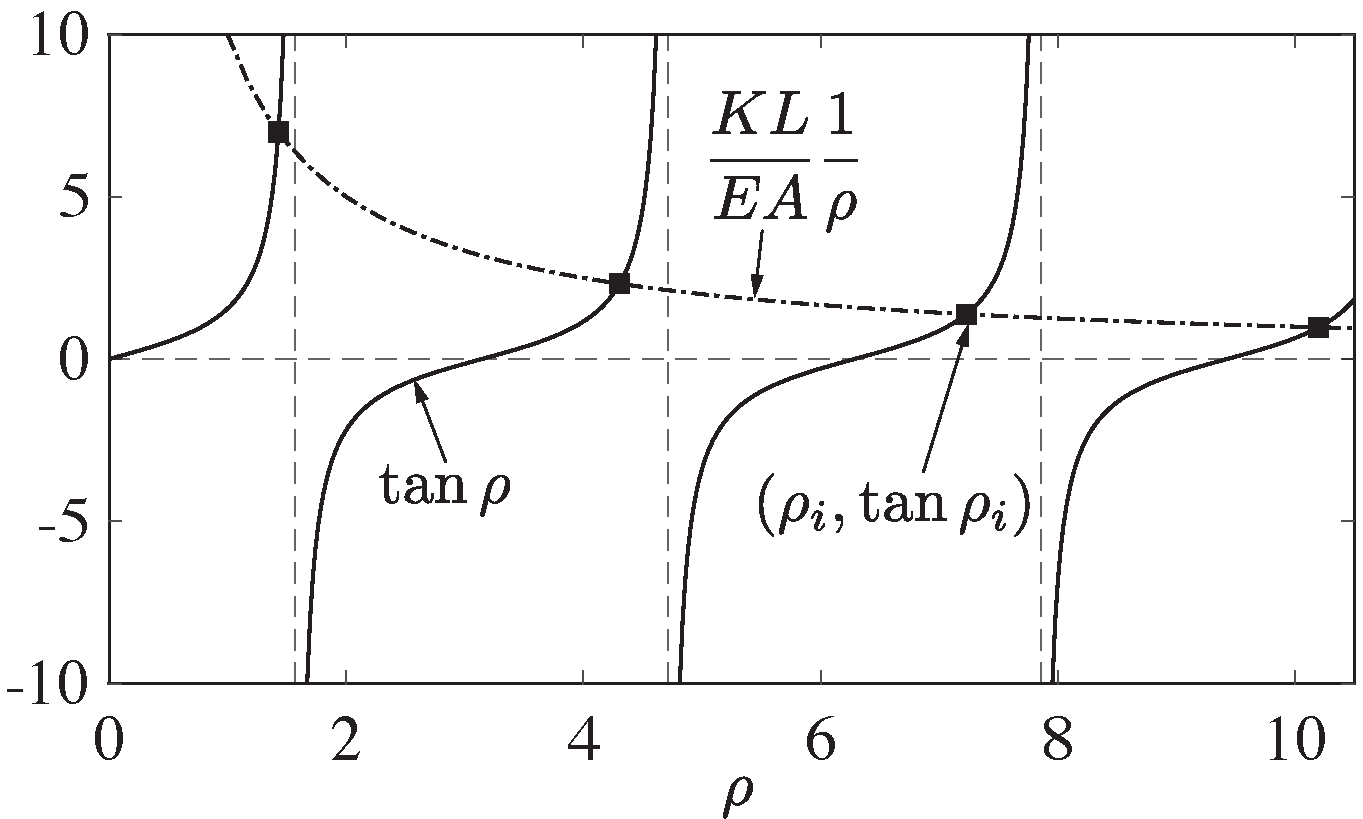
\includegraphics[width=0.5\textwidth]{homework/hw2/assets/hw2_p5_eval_eqn.pdf}
        \caption{Graphical representation of the eigenvalues \cref{eqn:hw2_p5_eval_eqn} as intersections between the tangent and the hyperbolic functions.}
        \label{fig:hw2_p5_eval_eqn}
    \end{figure}
}
\item { % 5(iii)
    In the limit of $K \rightarrow \infty$, the intersections behave as $\tan \rho \rightarrow \infty$, which corresponds to $\rho_n \rightarrow (n - 0.5)\pi$.
    This is identical to the eigenvalues in the \emph{free-fixed} boundary condition \emph{for the rod itself}.

    In the limit of $K \rightarrow 0$, the intersections behave as $\tan \rho \rightarrow 0$, which corresponds to $\rho_n \rightarrow n\pi$. 
    This is the same eigenvalues as \emph{free-free} boundary condition. 
    Moreover, the first eigenvalue move towards $\omega_i = 0$, which corresponds to a \emph{rigid body mode}. 

    Since $M$ does not factor into the eigenvalue equation \cref{eqn:hw3_p5_eigenvalue_eqn}, the spatial modes are unaffected by the change in $M$. 
    However, if one factor in the temporal modes, then it can be shown that as $M\rightarrow \infty$, the mass acts as a rigid wall and \emph{the entire system} behaves like a free-fixed rod (note the distinction from $K\rightarrow \infty$ case). 

    The above discussion, without considering temporal modes, is somewhat heuristic. 
    In (iv) we resolve the temporal modal oscillators which sheds more light on how the system behaves in these limits. 
}
\item { % 5(iv)
    Here we execute step (b) from part (i) where we find the temporal modes $\eta_i(t)$ based on the forced system. 
    Substituting the separable ansatz into the forced equations \cref{eqn:hw3_p5_eom_rod,eqn:hw3_p5_eom_mass} yields 
    \begin{subequations}
    \begin{align}
        \label{eqn:hw2_p5_eom_rod_sub} m\sum_{i=1}^\infty \varphi_i(x) \ddot{\eta}_i(t) &= EA\sum_{i=1}^\infty \left[ -\frac{\omega_i^2}{c^2} \varphi_i(x) \right] \eta_i(t) + Ky(t)\delta(x - L) \\
        \label{eqn:hw2_p5_eom_mass_sub} M \ddot{y}(t) &= -K \left[ y(t) - \sum_{i=1}^\infty \varphi_i(L) \eta_i(t) \right]
    \end{align}
    \end{subequations}
    Taking the inner product of \cref{eqn:hw2_p5_eom_rod_sub} with $\varphi_j(x)$ for some $j = 1, 2, 3, \ldots$ over $[0, L]$ leads to the modal oscillators for the rod:
    \begin{equation}\label{eqn:hw2_p5_modal_oscillators}
        \ddot{\eta}_j(t) + \omega_j^2 \eta_j(t) = K \varphi_j(L) y(t).
    \end{equation}
    \Cref{eqn:hw2_p5_eom_mass_sub,eqn:hw2_p5_modal_oscillators} can now be reorganized into a system of linear ODEs: 
    \begin{equation}
        \begin{bNiceArray}{cccc|c}[margin]
            1 & & & & 0  \\
            & \ddots & & & \vdots \\
            & & 1 & & 0   \\
            & & & \ddots & \vdots \\
            \hline
            0 & \cdots & 0 & \cdots  & M
        \end{bNiceArray}
        \begin{bNiceArray}{c}[margin]
            \ddot{\eta}_1(t) \\ 
            \vdots \\ 
            \ddot{\eta}_j(t)\\ 
            \vdots\\
            \hline
            \ddot{y}(t) 
        \end{bNiceArray} + 
        \begin{bNiceArray}{cccc|c}[margin]
            \omega_1^2 & & & & -K \varphi_1(L)  \\
            & \ddots & & & \vdots \\
            & & \omega_j^2 & & -K \varphi_j(L)  \\
            & & & \ddots & \vdots \\
            \hline
            \Block{1-4}{\textrm{symm.}} & & & & K
        \end{bNiceArray}
        \begin{bNiceArray}{c}[margin]
            \eta_1(t) \\ 
            \vdots \\ 
            \eta_j(t)\\ 
            \vdots\\
            \hline
            y(t) 
        \end{bNiceArray} = \bt{0}
    \end{equation}    
    or more compactly, 
    \begin{equation}\label{eqn:hw2_p5_modal_oscillator_matrix}
        \underbrace{\begin{bmatrix}
            \bt{I} & \bt{0} \\ 
            \bt{0} & M
        \end{bmatrix}}_{\bt{M}} 
        \underbrace{\begin{bmatrix}
            \ddot{\bv{\eta}}(t) \\ \ddot{y}(t)
        \end{bmatrix}}_{\ddot{\bv{v}}(t)} + 
        \underbrace{\begin{bmatrix}
            \bt{\Omega} & \bv{\psi} \\
            \bv{\psi}^T & K 
        \end{bmatrix}}_{\bt{K}} 
        \underbrace{\begin{bmatrix}
            \bv{\eta}(t) \\ y(t)
        \end{bmatrix}}_{\bv{v}(t)} = 0
    \end{equation}
    which is an $\infty$-DOF system. 
    However, it is often plausible to truncate the number of modes to a finite number $N$ (high frequency modes possess negligible energy), and obtain a finite-DOF system where $\bt{M}, \bt{K} \in \mathbb{R}^{(N+1)\times(N+1)}$.
    One can then treat this the same way as a discrete system via diagonalization:
    \begin{equation}
        \bt{K} \bt{Q} = \bt{M} \bt{Q} \bt{\Lambda}
    \end{equation}
    where $\bt{Q}$ is the matrix of eigenvectors and $\bt{\Lambda}$ is the diagonal matrix of eigenvalues. 
    In this system, both $\bt{K}$ and $\bt{M}$ are SPD (symmetric positive definite), which leads to a full set of real eigenpairs that can be chosen to satisfy the mass and stiffness ortho-normality conditions:
    \begin{equation}
        \bt{Q}^T \bt{M} \bt{Q} = \bt{I}, ~~~~ \bt{Q}^T \bt{K} \bt{Q} = \bt{\Lambda}.
    \end{equation}
    The system \cref{eqn:hw2_p5_modal_oscillator_matrix} is then decoupled as 
    \begin{equation}
        \ddot{\bv{w}}(t) + \bt{\Lambda} \bv{w}(t) = 0, ~~~~ \bv{v}(t) = \bt{Q} \bv{w}(t).
    \end{equation}
    The initial conditions are obtained as 
    \begin{equation}
        \eta_j(0) = \int_0^L m \varphi_j(x) U(x) dx, ~~~~ \dot{\eta}_j(0) = \int_0^L \varphi_j(x) V(x) dx, ~~~~ y(0) = \dot{y}(0) = 0,
    \end{equation}
    which constitutes the initial conditions of $\bv{v}(t)$.

    Finally, we reexamine some of the limits discussed in (iii). 
    Define gauge variable $\epsilon \ll 1$ and let subscripts denote asymptotic orders. 
    (For conciseness, some uses of symbols are cavalier.)
    \begin{enumerate}[(a)]
    \item {
        \emph{$K\rightarrow 0$}. 
        The system reads 
        \begin{equation}
            \begin{bmatrix}
                \bt{I} & \bt{0} \\ 
                \bt{0} & M
            \end{bmatrix} 
            \begin{bmatrix}
                \ddot{\bv{\eta}}(t) \\ \ddot{y}(t)
            \end{bmatrix} + 
            \begin{bmatrix}
                \bt{\Omega} & \epsilon \bv{\psi}_0 \\
                \epsilon \bv{\psi}_0^T & \epsilon K_0 
            \end{bmatrix}
            \begin{bmatrix}
                \bv{\eta}(t) \\ y(t)
            \end{bmatrix} = \bt{0}
        \end{equation}
        which implies the rod and the mass behaves independently on the leading order. 
        The mass's motion is oscillatory only at the first order. 
    } 
    \item {
        \emph{$K\rightarrow \infty$}. Multiplying both sides by $\epsilon$, the system becomes singularly perturbed:
        \begin{equation}
            \begin{bmatrix}
                \epsilon\bt{I} & \bt{0} \\ 
                \bt{0} & \epsilon M
            \end{bmatrix} 
            \begin{bmatrix}
                \ddot{\bv{\eta}}(t) \\ \ddot{y}(t)
            \end{bmatrix} + 
            \begin{bmatrix}
                \epsilon \bt{\Omega} & \bv{\psi}_0 \\
                \bv{\psi}_0^T & K_0 
            \end{bmatrix}
            \begin{bmatrix}
                \bv{\eta}(t) \\ y(t)
            \end{bmatrix} = \bt{0}
        \end{equation}
        which is not uniformly valid for all time. 
        Nonetheless, at leading order the scalar equation in $y(t)$ implies that the spring's deformation is small.
        This, in turn, suggests that the $u(L, t)$ is small if rigid body motion is suppressed (free-fixed BC). 
    }
    \item {
        \emph{$M\rightarrow \infty$}. Varying $M$ only affects the mass's equation:
        \begin{equation}
            \begin{bmatrix}
                \bt{I} & \bt{0} \\ 
                \bt{0} & M_0
            \end{bmatrix} 
            \begin{bmatrix}
                \ddot{\bv{\eta}}(t) \\ \ddot{y}(t)
            \end{bmatrix} + 
            \begin{bmatrix}
                \bt{\Omega} & \bv{\psi}_0 \\
                \epsilon \bv{\psi}_0^T & \epsilon K_0 
            \end{bmatrix}
            \begin{bmatrix}
                \bv{\eta}(t) \\ y(t)
            \end{bmatrix} = \bt{0}
        \end{equation}
        At the leading order, the mass maintains its velocity as its initial condition, which in this case is zero. 
        Hence, pictorially the mass acts like a rigid wall and the rod reduces to a free-spring system at the leading order.
    }
    \item {
        \emph{$M\rightarrow 0$}. Again the system becomes singularly perturbed:
        \begin{equation}
            \begin{bmatrix}
                \bt{I} & \bt{0} \\ 
                \bt{0} & \epsilon M_0
            \end{bmatrix} 
            \begin{bmatrix}
                \ddot{\bv{\eta}}(t) \\ \ddot{y}(t)
            \end{bmatrix} + 
            \begin{bmatrix}
                \bt{\Omega} & \bv{\psi}_0 \\
                \bv{\psi}_0^T & K_0 
            \end{bmatrix}
            \begin{bmatrix}
                \bv{\eta}(t) \\ y(t)
            \end{bmatrix} = \bt{0}
        \end{equation}
        At leading order, this again suggests that the spring barely deforms, and the rod behaves almost like a free-free system. 
    }
    \end{enumerate}
}
\end{enumerate}
